%%%%%%%%%%%%%%%%%%%%%%%%%
% Set up to be stand alone document
% All declerations in the header to be removed when added into thesis
%%%%%%%%%%%%%%%%%%%%%%%%%
\documentclass[12pt]{article}

\usepackage{booktabs} % booktabs provides professional formatting commands for tables
\usepackage{amsmath} % amsmath provides extra maths symbols
\usepackage{textcomp} % textcomp provides extra text symbols (like a degrees celsius symbol)
\usepackage{../customisations}

\title{J-band Sythentic Spectral Fitting}
\date{\today}

\begin{document}
\maketitle
%%%%%%%%%%%%%%%%%%%%%%%%%
% To be included when added into thesis
% \chapter{J-band Sythentic Spectral Fitting}

Based on the work done by Davies et al. (2010) and Gazak (2014), I developed an implementation of the J-band synthetic spectral fitting software.
This involves fitting the continuum between the observations and models and defining best fit model parameters for the stellar parameters,
metallicity, effective temperature, surface gravity and microturbulence.
The observations are fit with model spectra from a set of MARCS model atmospheres
\cite{2008A&A...486..951G}.
Spectra are extracted using the SUI code
~\cite{2012ApJ...751..156B,2013ApJ...764..115B,2014arXiv1412.6527B}
with non-LTE corrections computed for iron, silicon and titanium.

\subsection{Continuum Fitting} % (fold)
\label{sub:continuum_fitting}

Accurately matching the continuum levels in the models with that of the observed
spectrum provides a base with which to anchor the diagnostic lines.
An incorrecly placed continuum level would bias the analysis and result in the
strength of the diagnostic lines being over or under estimated producing inaccurate stellar parameters.

% The continuum fitting procedure is important because determining the base of the
% diagnostic lines defines their overall strength which is used to distinguish
% between models.
There are many factors that affect the level of the continuum and the continuum placement,
including the resolution of the observations as well as the stellar parameters themselves.
Therefore it is vital that when attempting to derive stellar paramters,
in crowded regions such as this, the continuum placement is performed
consistently and accurately.
Intrinsically, when stufying RSGs at medium resolution - owing  to their cool atmospheres -
there are may instances of blended spectral features.
At this resolution the density of spectral features creates a pseudo-continuum which in practice is never at the ture continnum level.
Figure~\ref{fig:mod-res} illustrates the varying continuum levels for models where the resolution is varied and
Figure~\ref{fig:mod-z} shows this affect when varying only the metallicity.

Given that it is impossible to know the true continuum level from any given observation,
any scaling applied must be consistent between the models and observations.
Scaling is required not only to match the levels of the continnum placement, but also to match the line strenghts between the models and observations.
Providing the treatment of the models and observations are consistent, the fact that the true continuum is never attained is not significant
\citep{2014ApJ...788...58G}.
For this procedure to work effectively, the observed and model spectra should be at the same resolution, have a consistent wavelength calibration and spectral sampling.

Each model spectrum is resampled onto the wavelength scale of the observations by means of a linear interpolation routine.
The model spectrum is then degraded to the resolution of the observations using a gaussian filter.
The resolution of the KMOS observations is estimated using the KMOS/esorex pipeline from arc lamp exposures at the appropriate rotator angle for the observations.
This is measured for each spectrograph and is assumed to be constant across individual IFU's as well as across the detector.

% This is accounted for by degrading the sampling of the models to that of the observations by means of a linear interpolation.
% The sampling of the models are degraded to that of the observations by means of a cublic-spline interpolation.
To ensure the spectra are on the same wavelength scale, the observed specturm is cross-correlated with the model spectrum;
a shift is then applied to the observed spectrum in order to minimise the cross-correlation matrix.
Over this small wavelength range, one would not expect significant variations in the spectral resolution of the observations to pertrub the cross-correlation.


\begin{figure}
 \centering
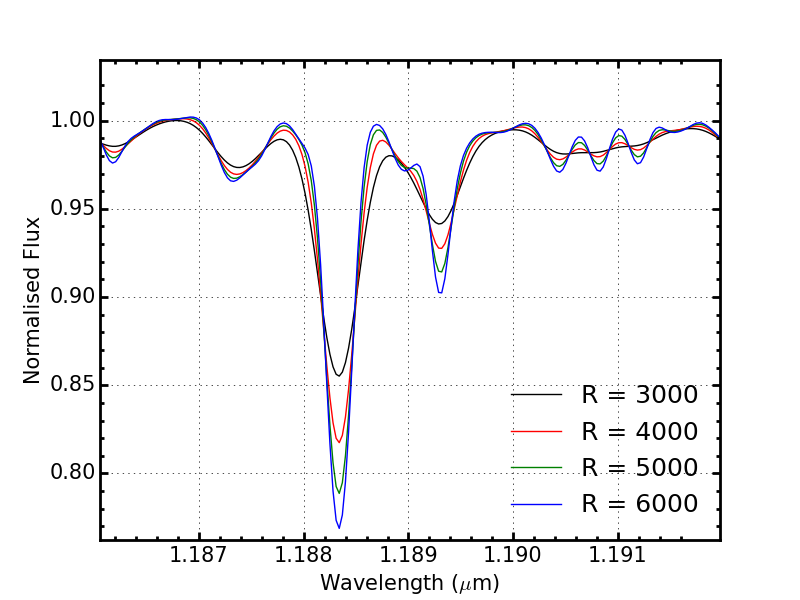
\includegraphics[width=\textwidth]{Resolution}
\caption{
Models at different resolutions.\label{fig:mod-res}
         }
\end{figure}


To fit the continuum of the observations first I define the continuum width ($cw$) as:

\begin{equation}
    cw = \frac{\lambda}{R}, %\times S,
\end{equation}
\noindent where $R$ is the resolution of the spectrum and
$\lambda$ is the wavelength at which the width is taken
(in principle this wavelength varies across the spectrum, however, given our spectral window is sufficently small, I assume $\lambda = 1.20\mu$m).
% and $S$ is a scale factor which takes the range $0.5 < S < 1.0$.
The continuum width is essentially the resolution element of the spectrum at a wavelength of $\lambda = 1.20\mu$m.
 % multiplied by the scale factor $S$.
% In Gazak et al. (2015) this scale factor is fixed at 0.5.
% The scale factor is introduced because ... ?

The model spectrum is divided into wavelength slices each of width $cw\mu$m and the maximum of each slice is taken.
Figure~\ref{fig:cw} illustrates that using this technique systematically removes absorption features from the spectrum.
In this figure blue points represent the boundaries between the slices of witdh $cw\mu$m and the maximum of each slice is shown in red.
Any remaining features in this maximum spectrum are removed by rejecting outliers which are more than 3$\sigma$ from the mean of the distribution.
In figure~\ref{fig:cw} the $cw~max.$ points have been through this procedure.
This can be seen by noting that the cores of the absorption lines no $cw max.$
points present.

\begin{figure}
 \centering
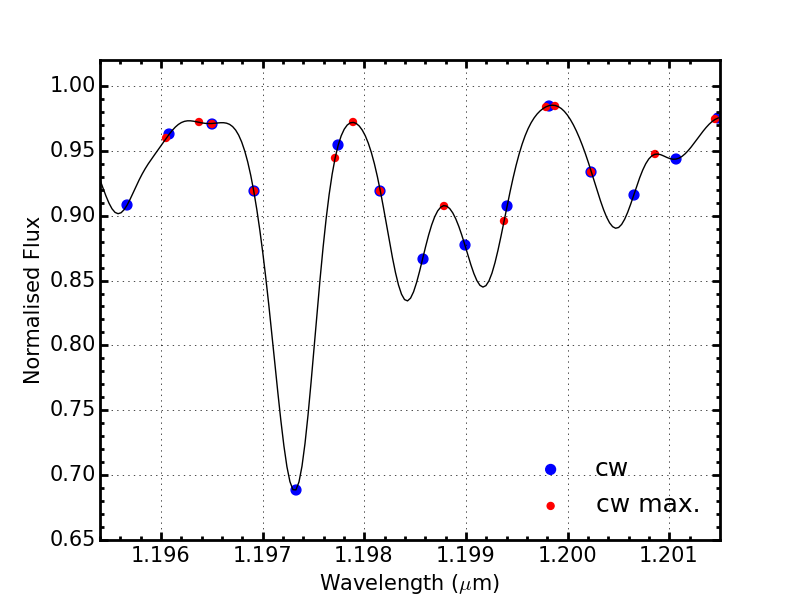
\includegraphics[width=\textwidth]{cw}
\caption{
Illustration of the continuum width ($cw$) and slicing the model spectrum into regions of $cw\mu$m is able to remove structure in order to fit the continnum.
The solid black line shows an example of a model spectrum degraded to a resolution of 3000,
blue points show the boundaries between the slices and red points show the maximum of each slice.\label{fig:cw}
         }
\end{figure}



The remaining data points ($P_{cont}$) are used to derive an inital correction function
($cf_{1}$) defined using the equation:
\begin{equation}
    cf_{1} = f(\frac{F_{mod}(P_{cont})}{F_{obs}(P_{cont})})
\end{equation}

\noindent where $F_{mod}$ and $F_{obs}$ are the flux in the model and observed spectrum respectively.
The final correction function ($cf_{2}$), a refinement of $cf_{1}$,
is defined by removing outliers more than 3$\sigma$ from the mean of the correction function $cf_{1}$.
This function is used to define the amount of scaling required for the model.


% The green dashed line shows a third order polynomial fit to the ratio of the model spectrum to a simulated observed spectrum at only the red points ($ = \frac{F_{mod}(cf_{1})}{F_{obs}(cf_{1})}$).


Alternative methods of continuum fitting are discussed in~\cite{2010MNRAS.407.1203D} and~\cite{2011A&A...527A..50E}.
These methods select pseduo-continuum pixels in the models based on ranking the model pixels and selecting a percentage of the pixels with the largest flux.
Providing the pixels from the model are selected in this manor and not those in the observations, this is a reliable method with which to derive the continuum level as demonstrated by Davies et al. (2015 in prep.).
\textbf{What advantage (if any) does the method applied here have over the one used in Davies et al. (2015 in prep.)?}

% subsection continuum_fitting (end)
\subsection{Best Fit Parameters} % (fold)
\label{sub:best_fit_parameters}

Bestfit paramaters are calcaulted using a chi-squared minimisation approach.
Each model in a 40,000 strong model grid is compared to the observed spectrum
and a chi-squared value is calculated using the equation,

\begin{equation}
    \chi^{2} = \sum{\frac{(O_{i} - M_{i})^{2}}{\sigma^{2}}}
\end{equation}

% subsection best_fit_parameters (end)
\bibliography{../journals}
%%%%%%%%%%%%%%%%%%%%%%%%%
% To be removed when added into thesis
\end{document}
%%%%%%%%%%%%%%%%%%%%%%%%%